\documentclass[a4paper,12pt]{article}

% Packages
\usepackage[utf8]{inputenc}
\usepackage{amsmath, amssymb}
\usepackage{graphicx}
\usepackage{float} % Required for [H] specifier in figures
\usepackage{hyperref}
\usepackage{geometry}
\usepackage{textcomp} % For \textdegree command
\usepackage{indentfirst}
\usepackage{caption}
\usepackage{tabularx} % Add this to the preamble if not already included
\usepackage{subcaption} % Required for subfigure environment
\usepackage[backend=biber]{biblatex}
\addbibresource{references.bib} % Name of your .bib file
\geometry{margin=1in}



% Title and Author
\title{Zeeman Effect}
\author{Henry Su, Wen Hong Lou\\ NTU Physics Department}
\date{\today}

\begin{document}

\maketitle

\begin{abstract}
This report investigates the Zeeman Effect, a phenomenon where spectral lines are split into multiple components in the presence of a magnetic field. The experiment aims to measure the splitting and verify the theoretical predictions. 
\end{abstract}

\tableofcontents
\newpage

\section{Introduction}
The Zeeman effect, discovered by Pieter Zeeman in 1896, is the splitting of atomic spectral lines in the presence of a magnetic field. This experiment investigates both the normal and anomalous Zeeman effects, demonstrating how magnetic fields influence atomic energy levels. Using a cadmium lamp and a Fabry-Perot interferometer, we will observe the shifts in wavelength caused by the interaction of electron magnetic moments with an external magnetic field. Additionally, we will calculate the Bohr magneton, a fundamental physical constant that quantifies the magnetic moment of an electron due to its orbital or spin motion. This study enhances our understanding of atomic structure and the fundamental principles of quantum mechanics.\section{Theory}
\subsection{Zeeman Effect}
Zeeman effect is a phenomenon that an atomic spectral line is split into several components in the presence of a magnetic field. The splitting occurs due to the interaction between the magnetic moment of the atom and the external magnetic field. The effect can be classified into two types: normal and anomalous Zeeman effects. We'll get into the details of these two types in the latter section. But for now let us focus on the basic theory of the Zeeman effect. In the presence of weak magnetic field $\mathrm{B}$ the perturbed Hamiltonian can be written as follows:
\begin{equation}
H' = -\mathbf{\mu} \cdot \mathbf{B} = -\mu_B \mathbf{J} \cdot \mathbf{B} , ~~~ \mu_B = \frac{e \hbar}{2 m_e} = 9.274 \times 10^{-24} \mathrm{J/T}
\end{equation}
where $\vec{\mu}$ is the magnetic moment, $\mu_B$ is the Bohr magneton, and $\bold{J}$ is the total angular momentum of the atom. In particular, $\bold{J} = \bold{L} + 2\bold{S}$ where the factor 2 is the g-factor for the electron spin. In the latter on experiments our goal is to calculate Bohr magneton through energy level spliting. \\
\indent  Now let's consider the energy of the perturbed Hamiltonian by firt order perturbation theory. The "good state" of the perturtion is the normalized eigenbasis of the unperturbed Hamiltonian($H_0$), and it's charaterized mainly by magnetic quantum number $m_j$ and orbital quantum number $\ell$. With $\bold{B} = \mathrm{B}\hat{z}$, the energy of the perturbed Hamiltonian can be written as: 
\begin{align}
    E_{mj} 
    &= \langle n \ell jm_j \mid H' \mid n\ell jm_j \rangle \\
    &= \mu_{B}\,B \biggl[
      1 + \frac{j\,(j+1) + s\,(s+1) - l\,(l+1)}{2\,j\,(j+1)}
    \biggr] \, m_{j} 
    = -\,g_j\,\mu_{B}\,B\,m_{j}.
    \label{eq:zeeman_energy}
\end{align}
where $g_j$ is the Landé g-factor.
\subsection{Selection Rules}
Dispite knowing physically all the possible energy level existed, naturally not all transitions between state is allowed. We know the selection rule coonstrains the possible transitions between these energy states. There are two types of transitions allowed: 
\begin{align}
    \text{$\pi$-line : }&\Delta m_j = \pm 1\\ 
    \text{$\sigma_{\pm}$-line : }&\Delta m_j = 0 
\end{align}
\indent In our experimentm, we detected lights propagating parellel and perpendicular to the magnetic field $\bold{\mathrm{B}}$. Furthermore, the corrsponding two types of transitions to the light propagatind directions can be summurized in Fig.\ref{fig:zeeman_effect_1}
\begin{figure}[H] % Ensure [H] is used correctly with the float package
    \centering
    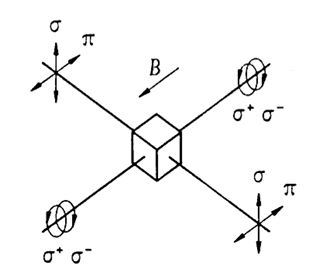
\includegraphics[width=0.5\textwidth]{Zeeman_effect_1.png}
    \caption{Illustration of the allowed transitions for the Zeeman effect, showing $\pi$-lines ($\Delta m_j = 0$) and $\sigma$-lines ($\Delta m_j = \pm 1$) for light propagating perpendicular to the magnetic field. Note that there is no $\pi$-line for light propagating parallel to the magnetic field because the magnetic dipole is oriented along the field. \cite{phyweZeeman}}
    \label{fig:zeeman_effect_1}
\end{figure}

\subsection{Normal and Anomalous Zeeman Effect}
The primary distinction between the normal and anomalous Zeeman effects lies in the electron spin. For the normal Zeeman effect, the electron spin $s = 0$, whereas for the anomalous Zeeman effect, $s \neq 0$. 

In terms of transitions, the initial state can be represented as $\mid i \rangle = \mid \ell_i, s_i, j_i, m_{j_i} \rangle$, and the final state as $\mid f \rangle = \mid \ell_f, s_f, j_f, m_{j_f} \rangle$. In our experiment, we use cadmium, and the specific transitions for the normal and anomalous Zeeman effects are as follows:
\begin{align}
    \text{Normal: } & \, 3^1\mathrm{D_2} \to 2^1\mathrm{P_1} \quad \text{or} \quad \mid 3; 2, 0, 2, m_j \rangle \to \mid 2; 1, 0, 1, m_j \rangle, \\
    \text{Anomalous: } & \, 2^3\mathrm{S_1} \to 2^3\mathrm{P_2} \quad \text{or} \quad \mid 2; 0, 1, 1, m_j \rangle \to \mid 2; 1, 1, 2, m_j \rangle.
    \label{eq:zeeman_transitions}
\end{align}
Indeed this form of transition representation loses the information of quantum number $m_j$. However, that's a not a big deal since later we only care about the $\Delta m_j$. So going back to the enegry difference between transions, we can use eq.\ref{eq:zeeman_energy} to calculate the energy difference between the two transitions as:
\begin{align}
    \Delta E &= \Delta E_0 + \mu_B B \biggl[ g_{j_f} m_{j_f} - g_{j_i} m_{j_i} \biggr], \,
    \begin{cases}
        \Delta m_{j} = m_{j_f} - m_{j_i} = 0, \, \text{for } \pi \text{-line} \\
        \Delta m_{j} = m_{j_f} - m_{j_i} = \pm 1, \, \text{for } \sigma_{\pm} \text{-line}
    \end{cases}
\end{align}
with the plotting corresponding quantum number in Eq.~\ref{eq:zeeman_transitions}, we have,
\begin{align}
    \begin{cases} 
        \text{Normal: } g_{j_f} = g_{j_i} = 1, \, \Delta m_j = m_{j_f} - m_{j_i}, \\
        \text{Anomalous: } g_{j_i} = 2, \, g_{j_f} = \frac{3}{2}
    \end{cases}
\end{align}
\indent Then we can summarize the transitions in Fig.~\ref{fig:zeeman_comparison}.

\begin{figure}[H]
    \centering
    \begin{subfigure}[b]{0.45\textwidth}
        \centering
        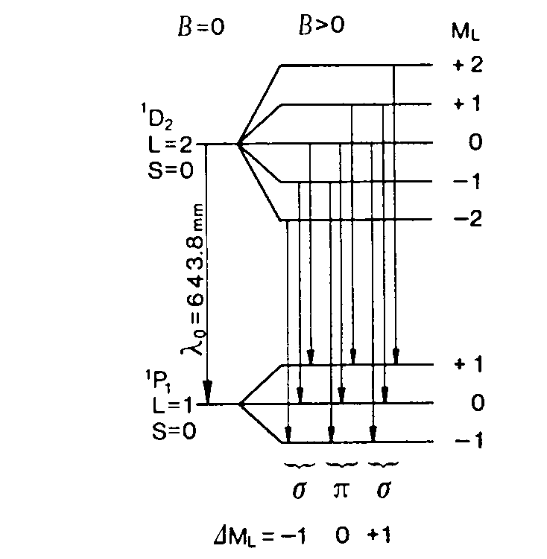
\includegraphics[width=\textwidth]{Normal_Zeeman.png}
        \caption{Normal Zeeman Transitions}
        \label{fig:normal_zeeman}
    \end{subfigure}
    \hfill
    \begin{subfigure}[b]{0.45\textwidth}
        \centering
        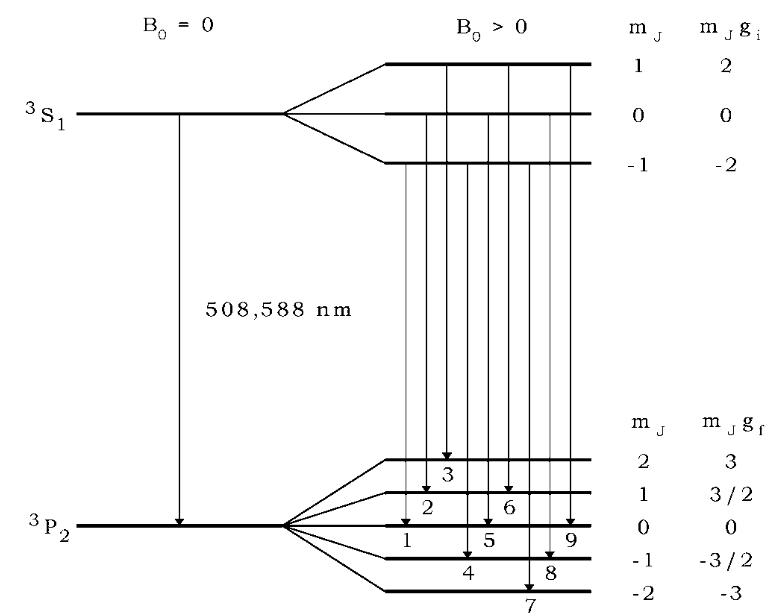
\includegraphics[width=\textwidth]{Anomalous_Zeeman.png}
        \caption{Anomalous Zeeman Transitions}
        \label{fig:anomalous_zeeman}
    \end{subfigure}
    \caption{Transitions we use for cadmium in our experiment. Theoretically, there are nine possible transition states for both effects. However, after passing through the Fabry-Perot Étalon, some transitions fail to exist.\cite{phyweZeeman}}
    \label{fig:zeeman_comparison}
\end{figure}
\subsection{Fabry-Perot Etalon: Frequency Selection}
The Fabry-Perot etalon is a critical component in our experiment, used to select specific frequencies from the light emitted by the cadmium lamp. Since the light source is not monochromatic, the etalon ensures that only the desired spectral lines are transmitted for analysis.

The etalon consists of two parallel, partially reflecting mirrors separated by a distance $d$. Light waves reflect back and forth between the mirrors, creating an interference pattern. The condition for constructive interference is given by:
\begin{equation}
    2\mu t\cos \theta = n \lambda,
\label{eq:fabry_perot_condition}
\end{equation}
where $t$ is the separation between the mirrors, $\theta$ is the angle of incidence, $n$ is the interference order, $\mu$ is the reflective index in quartz, and $\lambda$ is the wavelength of the transmitted light. 


Figure \ref{fig:fabry_perot_interference} illustrates the working principle of the Fabry-Perot etalon. Light entering the etalon at an angle $\theta$ undergoes multiple reflections, and only wavelengths satisfying the interference condition (eq.\ref{eq:fabry_perot_condition}) emerge constructively. Thus we have:
\begin{equation}
    n = \frac{2\mu t}{\lambda} \cos \theta_n = n_0 \cos \theta_n, \quad \text{where } n_0 = \frac{2\mu t}{\lambda}.
\end{equation}

\begin{equation}
    \theta_n = \sqrt{\frac{2(n_{0}-n)}{n_{0}}}
\end{equation}
\begin{figure}[H]
    \centering
    \begin{subfigure}[b]{0.45\textwidth}
        \centering
        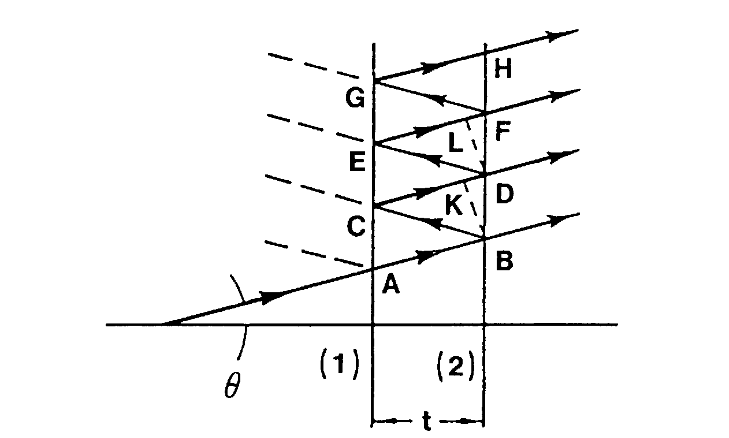
\includegraphics[width=\textwidth]{fabry_perot_2.png}
        \caption{Reflected and transmitted rays at the parallel surfaces.}
        \label{fig:fabry_perot_interference}
    \end{subfigure}
    \hfill
    \begin{subfigure}[b]{0.45\textwidth}
            \centering
            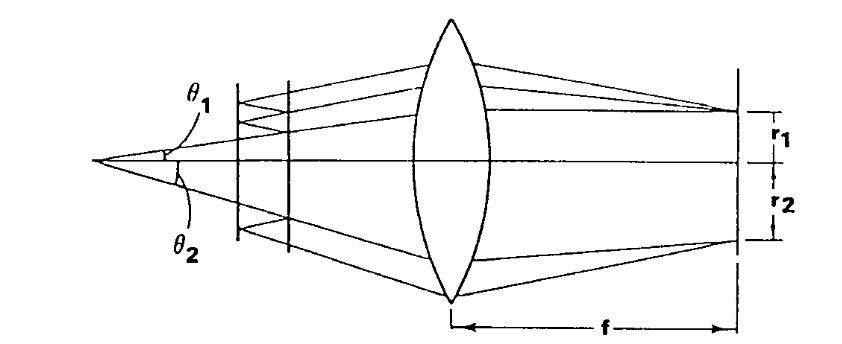
\includegraphics[width=\textwidth]{fabry_perot_1.png}
            \caption{Ring radius on the analyser is $r = f\theta$, where $f$ is the focal length of the lens.}
            \label{fig:fabry_perot_focusing}
        \label{fig:fabry_perot_focusing}
    \end{subfigure}
    \label{fig:fabry_perot_diagram}
\end{figure}
\indent And since $n_1 < n_0$ and $n_1 = n_0 \cos \theta$, we can let:
\begin{equation}
    n_1 = n_0 - \epsilon \quad ; 0<\epsilon < 1
\end{equation}
\indent And for the pth order of interference, we have:
\begin{equation}
    n_p = (n_0 - \epsilon) - (n_p -1)
\end{equation}
\indent We can see in figure \ref{fig:fabry_perot_focusing} that the light rays are focused on the analyser. With small angle approximation, we can write the radius of the ring on the analyser as:
\begin{equation}
    r = f \tan\theta \approx f \theta
    \label{eq:fabry_perot_radius}
\end{equation}
\indent Therefore, combining eq.\ref{eq:fabry_perot_condition} and eq.\ref{eq:fabry_perot_radius}, we can get the difference on radius of the ring on the analyser as:
\begin{equation}
     r^2_{p+1} - r^2_{p} = 2 \frac{f^2}{n_0}, ~~~\,\text{with}\, r_p = \sqrt{\frac{2f^2}{n_0}} \cdot \sqrt{(p-1) + \epsilon} 
    \label{eq:fabry_perot_radius_diff}
\end{equation}
\indent Now if there are two different wavelengths $\lambda_a$ and $\lambda_b$ in the light source, we can write the $n_0$ for both wavelengths respect to its corresponding wave number $k_a$ and $k_b$ as:
\begin{align}
    \begin{cases}
        \epsilon_a &= \frac{2\mu \cdot t}{\lambda_a} = -n_{1,a} = 2\mu \cdot t \cdot k_a - n_{1,a}, \\
        \epsilon_b &= \frac{2\mu \cdot t}{\lambda_b} = -n_{1,b} = 2\mu \cdot t \cdot k_b - n_{1,b}.
    \end{cases}
    \label{eq:fractional_orders}
\end{align}
\indent Then combining eq.\ref{eq:fabry_perot_radius_diff} and eq.\ref{eq:fractional_orders}, we can get the difference of wave number $k$ as:
\begin{align}
    \Delta k &= k_a - k_b = \frac{1}{2\mu \cdot t} \biggl[ \frac{r_{p+1,a}^2}{r_{p+1,b}^2 - r_{p,a}^2} - \frac{r_{p+1,b}^2}{r_{p+1,b}^2 - r_{p,b}^2} \biggr]
    \label{eq:wave_number_diff}
\end{align}
\indent From the relation in eq.\ref{eq:fabry_perot_radius}, we can assume for $n_{0,b} \approx n_{0,a}$ we have:
\begin{equation}
    \Delta^{p+1,p}_{a} = r^2_{p+1} - r^2_{p,a} = 2 \frac{f^2}{n_{0,a}} = \Delta^{p+1,p}_{b} = r^2_{p+1} - r^2_{p,b} = 2 \frac{f^2}{n_{0,b}}
\end{equation}
\indent and for all value of $p$ we have: 
\begin{equation}
    \delta^{p}_{a} = r^2_{p+1,a} - r^2_{p+1,a} 
\end{equation}
\indent Thus, we rewrite eq.\ref{eq:wave_number_diff} as(assuming $\Delta E_0 = 0$):
\begin{equation}
    \Delta k = \frac{1}{2\mu \cdot t}\cdot\frac{\delta}{\Delta}
    \label{eq:wave_number_diff_final}
\end{equation}
\indent From the above we can reqrite the energy differnce in terms of $\Delta k$:
\begin{equation}
    \Delta E = \mu_B B \biggl[ g_{j_f} m_{j_f} - g_{j_i} m_{j_i} \biggr] =  \hbar c \Delta k = \frac{\hbar c}{2\mu \cdot t} \cdot \frac{\delta}{\Delta}
    \label{eq:energy_diff_final}
\end{equation}
To summarize, we can see the possible rings in given $p$ in table.\ref{tab:ZeemanComparison}
\begin{table}[ht]
    \centering
    \renewcommand{\arraystretch}{1.2}
    \begin{tabular}{c|c|c}
    \hline
     & (a) $\Delta\bigl(g_j m_j\bigr)$ 
     & (b) Possible rings for a fixed order \\
    \hline
    \textbf{Normal} 
     & \begin{tabular}{@{}l@{}}
       $\sigma(\Delta m_j = +1): \{+1,+1,+1\}$\\
       $\sigma(\Delta m_j = -1): \{-1,-1,-1\}$\\
       $\pi(\Delta m_j = 0): \{0,0,0\}$\\
       \end{tabular}
     & \begin{tabular}{@{}l@{}}
       \textit{Transverse}: 1 + 2 rings \\
       \textit{Longitudinal}: 0 + 2 rings
       \end{tabular}
    \\
    \hline
    \textbf{Anomalous} 
     & \begin{tabular}{@{}l@{}}
       $\sigma(\Delta m_j = +1): \{2,\tfrac{3}{2},1\}$\\
       $\sigma(\Delta m_j = -1): \{-\tfrac{3}{2},-1,-\tfrac{1}{2}\}$\\
       $\pi(\Delta m_j = 0): \{\tfrac{1}{2},0,-\tfrac{1}{2}\}$\\
       \end{tabular}
     & \begin{tabular}{@{}l@{}}
       \textit{Transverse}: 3 + 6 rings \\
       \textit{Longitudinal}: 0 + 6 rings
       \end{tabular}
    \\
    \hline
    \end{tabular}
    \caption{(a) The value of $\Delta\bigl(g_j m_j\bigr)$ for normal and anomalous Zeeman effects, and 
    (b) the corresponding number of rings in the Fabry--Perot interference pattern for a fixed order with the left number representing $\pi$-line and right number representing $\sigma_{\pm}$.}
    \label{tab:ZeemanComparison}
    \end{table}
    

\section{Experiment Setup and Procedure}
\subsection{Experimental Setup}
The electromagnet is placed on a rotating table designed for heavy loads and is mounted with two pole-pieces that have holes, leaving a gap (9--11~mm) large enough for the Cd-lamp. The pole-pieces must be tightened securely. The Cd-lamp is inserted into the gap without touching the pole-pieces and is connected to the power supply for spectral lamps.

The scheme of the set up can be shown in figure.\ref{fig:setup}.
\begin{figure}[H]
    \centering
    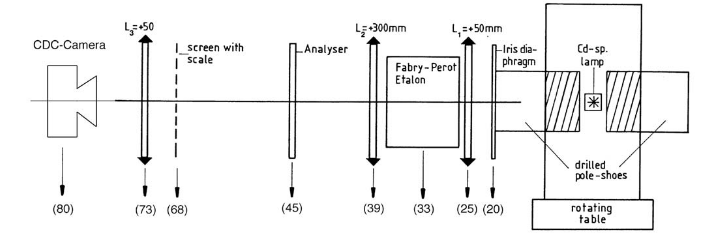
\includegraphics[width=0.8\textwidth]{setup.png}
    \caption{Experimental setup for observing the Zeeman effect. The optical bench is equipped with a lens system, a Fabry-Perot étalon, and a CCD camera for capturing the interference pattern.}
    \label{fig:setup}
\end{figure}
\subsection{Procedure}
    1. First we open the cadmium light and put on the red light filter make sure that the fringes on the CCD is center at the center of the screen. \\
\indent 2. Then we adjust the Fabry-Perot etalon to get the best interference pattern. The etalon is adjusted by rotating the two screws on the side of the etalon. The best interference pattern is achieved when the rings are sharp and well-defined. We also change focals and exposure of the CCD to get the best resolution\\
\indent 3. After that we took picture of the polarization entering the CCD at 0\textdegree, 90\textdegree, and 180\textdegree\\ 
\indent 4. Then we rotate the electromagnet by 90\textdegree, insert quarter waveplate and replace the red light filter with green light filter for longitudinal observation.\\
\indent 5. We repeat the same procedure as above to get the best interference pattern.\\
\indent 6. After that we took picture of the polarization entering the CCD at 0\textdegree, 90\textdegree, and 180\textdegree\\

\subsection{Transversal Observation}
    After completing the initial adjustments, the electromagnet is rotated by 90\textdegree, and the iris diaphragm is inserted for transversal observation.
    
    \subsection{Calibration Remark}
    For later evaluations, a calibration curve of the magnetic flux density versus the coil current must be recorded. This can be performed using a teslameter. If unavailable, the results shown in Fig.~3 can be used. Note that the flux density measured in the center of the gap (in the absence of the Cd-lamp) should be increased by 3.5\% to account for the non-uniform flux distribution within the gap.
    
    % End of Section 3
    

\section{Results}
Present the observed spectral line splitting and compare it with theoretical predictions. Include tables and graphs where necessary.

\section{Discussion}
Analyze the results, discuss sources of error, and evaluate the agreement between experimental and theoretical values.

\section{Conclusion}
Summarize the findings and their implications for understanding the Zeeman Effect.

\section*{References}
\printbibliography

\end{document}